\documentclass{math}

\usepackage{tikz}
\usetikzlibrary{arrows}

\title{Introduction to Computer Science Theory}
\author{Alvin Lin}
\date{August 2017 - December 2017}

\begin{document}

\maketitle

\section*{Abstract Machines}
Our goal is to answer fundamental computer science questions:
\begin{itemize}
  \item What can and cannot be computed?
  \item What can and cannot be computer efficiently?
\end{itemize}
To answer this, we need a \textbf{universal model of computation}. We also need
\textbf{restricted models of computation}, such as string matching, lexical
analysis, and parsing.

\subsection*{Finite Automata}
This is our most restricted model, and it can be represented as input on tape
that reads input once from left to right. It has no memory except for one
register.
\[ \texttt{[a a b a c a d a b a d a]} \]
They have finite control and contain a state. We call these
\textbf{deterministic finite automata}.

\subsection*{What languages can finite automatons recognize?}
Given a language, we want to write a program that given a string, can tell
whether or not the string is in the language. For this example, we will define
our language as the strings over \( \{a,b\} \) that contain an even number of
\( a \)'s.
\[ \{aab,aba,aa,b,\epsilon\}\in L \]
\[ \{ab,a,abb\}\notin L \]
One algorithm:
\begin{itemize}
  \item Let \( n_a \leftarrow 0 \)
  \item For \( i\in\{1,\dots,n\} \): If \( x_i == a \), let \( n_a\leftarrow
  n_a+1 \).
  \item If \( n_a \) is even, accept.
  \item Else, reject.
\end{itemize}
This algorithm cannot be run on a finite automaton because the \( n_a \)
counter can get arbitrarily large. A finite automata can only have a finite
number of states.

\subsubsection*{Example}
Give \textbf{set builder notation} and a \textbf{transition diagram} for a
finite automaton that recognizes the language that consists of the strings over
\( \{a,b\} \) that:
\begin{itemize}
  \item contain an even number of \( a \)'s.
  \[ \{x\in\{a,b\}^*\mid x\ has\ 0\ mod\ 2\ a's \} \]
  \begin{center}
    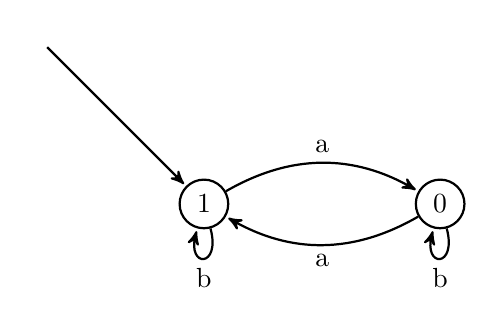
\begin{tikzpicture}[->,>=stealth',shorten >=1pt,auto,node distance=3cm,
                        thick]
      \node[circle,draw] (0) {0};
      \node[circle,draw] (1) [left of=0] {1};
      \node (2) [above left of=1] {};
      \path (2) edge (1)
        (0) edge[loop below] node {b} (0) edge[bend left] node {a} (1)
        (1) edge[loop below] node {b} (1) edge[bend left] node {a} (0);
    \end{tikzpicture}
  \end{center}
  \item contain at least 3 \( a \)'s.
  \begin{center}
    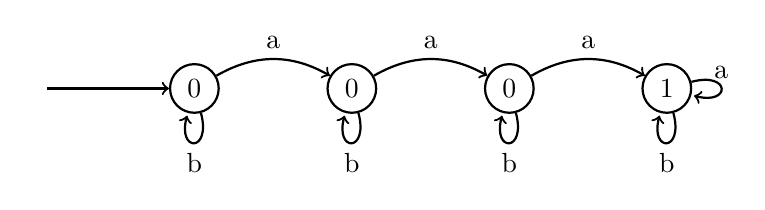
\begin{tikzpicture}[->,node distance=2cm,thick]
      \node[circle,draw] (0) {0};
      \node[circle,draw] (1) [right of=0] {0};
      \node[circle,draw] (2) [right of=1] {0};
      \node[circle,draw] (3) [right of=2] {1};
      \node (4) [left of=0] {};
      \path (4) edge (0)
        (0) edge[loop below] node {b} (0) edge[bend left] node[above] {a} (1)
        (1) edge[loop below] node {b} (1) edge[bend left] node[above] {a} (2)
        (2) edge[loop below] node {b} (1) edge[bend left] node[above] {a} (3)
        (3) edge[loop below] node {b} (3) edge[loop right] node[above] {a} (3);
    \end{tikzpicture}
  \end{center}
\end{itemize}
Formally defined, a finite automata is a quintuple \( M =
(Q,\Sigma,\delta,q_0,F) \), where:
\begin{itemize}
  \item \( Q \) is a finite set of \textit{states}
  \item \( \Sigma \) is an alphabet of \textit{input symbols}
  \item \( \delta \) is a total function from \( Q\times\Sigma \) to \( Q \):
    the \textit{transition function} (\( \delta \) is often given as a
    \textit{transition table})
  \item \( q_0\in Q \) is the \textit{initial state}
  \item \( F\subseteq Q \) is the set of \textit{accepting} states
\end{itemize}
For the example above of a finite automaton that contains an even number of
\( a \)'s: \( M = (Q,\Sigma,\delta,0,\{0\}) \), where:
\begin{itemize}
  \item \( Q = \{0,1\} \)
  \item \( \Sigma = \{a,b\} \)
  \item \( \delta \): \( Q\times\Sigma\to Q \) is defined on \( (q,z)\in
    Q\times\Sigma \) as:
    \[ \delta(q,x) = \begin{cases}
      q & if\ x = b \\
      q+1\mod2 & otherwise
    \end{cases} \]
\end{itemize}

\subsection*{Acceptance on Deterministic Finite Automata}
For finite automaton \( M = (Q,\Sigma,\delta,q_{\circ},F) \), \( \delta(q,a) \)
is the state \( M \) goes to if it is in state \( q \) and reads an \( a \).
We say that \( M \) accepts \( w = w_1w_2\dots w_n\in\Sigma^{*} \) if there is
a sequence (repeats allowed) of states \( r_0,r_1,\dots,r_n\in Q \) such that:
\begin{enumerate}
  \item \( r_0 = q_0 \)
  \item \( \forall{i}\in\{0,\dots,n-1\}(\delta(r_i,w_{i+1} = r_i+1) \)
  \item \( r_n \in F \)
\end{enumerate}
A deterministic finite automaton \( M \) recognizes a language \( A \) if
\( A = \{w\mid M\ accepts\ w\} \). We say \( A = L(M) \). A language is called
a \textbf{regular language} if some finite automaton recognizes it.

\subsection*{Nondeterminism}
Look at the following transition diagram for the set of strings over \( \{a,b\}
\) that contain at most 2 \( a \)'s.
\begin{center}
  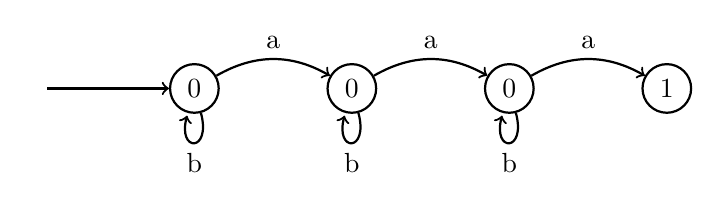
\begin{tikzpicture}[->,node distance=2cm,thick]
    \node[circle,draw] (0) {0};
    \node[circle,draw] (1) [right of=0] {0};
    \node[circle,draw] (2) [right of=1] {0};
    \node[circle,draw] (3) [right of=2] {1};
    \node (4) [left of=0] {};
    \path (4) edge (0)
      (0) edge[loop below] node {b} (0) edge[bend left] node[above] {a} (1)
      (1) edge[loop below] node {b} (1) edge[bend left] node[above] {a} (2)
      (2) edge[loop below] node {b} (1) edge[bend left] node[above] {a} (3);
  \end{tikzpicture}
\end{center}
This is not the transition diagram of a finite automaton because the last state
is missing transitions. Nondeterminism removes the restrictions on finite
automata and allows for a transition diagram to omit transitions on certain
inputs or multiple transitions on certain inputs. Formally defined, a
nondeterministic finite automaton is a quintuple \( M = (Q,\Sigma,\delta,
q_0,F) \) where:
\begin{itemize}
  \item \( Q \) is a finite set of \textit{states}
  \item \( \Sigma \) is an alphabet of \textit{input symbols}
  \item \( \delta \) is a total function from \( Q\times\Sigma_{\epsilon} \) to
  \( 2^Q \)
  \item \( q_0 \) is the initial state
  \item \( F\subseteq Q \) is the set of \textit{accepting states}
\end{itemize}

\subsection*{Acceptance on Nondeterministic Finite Automata}
For finite automaton \( M = (Q,\Sigma,\delta,q_0,F) \), \( \delta(q,a) \)
is the state \( M \) goes to if it is in state \( q \) and reads an input
\( a \). We say that \( M \) accepts \( w = w_1w_2\dots w_n \) where each
\( w_i\in\Sigma_{\epsilon} \) if there is a sequence of states \( r_0,r_1,
\dots,r_n\in Q \) such that:
\begin{itemize}
  \item \( r_0 = q_0 \)
  \item \( \forall{i}\in\{0,\dots,n-1\}(r_{i+1}\in\delta(r_i,w_{i+1})) \)
  \item \( r_n\in F \)
\end{itemize}

\begin{center}
  You can find all my notes at \url{http://omgimanerd.tech/notes}. If you have
  any questions, comments, or concerns, please contact me at
  alvin@omgimanerd.tech
\end{center}

\end{document}
